\documentclass[12pt]{article}
\usepackage{graphicx}
\usepackage{pdfpages}
\usepackage{hyperref}
\usepackage[margin=1in]{geometry}
\usepackage[utf8]{inputenc}
\graphicspath{ {./Figures/} }
\hypersetup{
    colorlinks=true,
    linkcolor=blue,
    filecolor=magenta,      
    urlcolor=cyan,
}
\urlstyle{same}
\usepackage[font={tiny,it}]{caption}
\usepackage{fancyvrb}
\title{Analysis, Visualization, \& Simulation of South Bend Government Call Center}
\author{John D. Bulger \& Karl R.B. Schmitt\\
	Mathematics \& Statistics Department\\
	Affiliate, Computing \& Information Sciences Department
	\\Valparaiso University, Valparaiso, IN}
\date{March 10, 2019}

	\begin{document}
\maketitle
\section{Introduction}
The city of South Bend, located in northern Indiana, established a citizen-accessible call center in February 2013.  It addresses almost every aspect of city-citizen interaction, including waste pick-up and removal, water billing and disconnections, and code enforcement.  By serving as a central hub for communication, the call center is able to consolidate a substantial amount of data regarding citizens as consumers.  This data is available on South Bend's open data portal at \textit{https://data-southbend.opendata.arcgis.com}.

\subsection{Goals \& Desired Results}

% Clean up and put stuff here

\section{Prior Work}
	
Efficiency and success of a call center can be measured by different metrics.  Baraka identifies success principles such as customer satisfaction, service quality, and usage amount, while specifically suggesting call duration as a quantifiable, key metric \cite{baraka}. Other work on call centers have focused on first call resolution (“FCR”), customer satisfaction, and operator tenure as a key metrics, albeit with differing analytical goals.  Chen et al. use FCR in order to analyze call center efficiency utilizing rough set theory \cite{chen}. Within in the scope of this paper’s analysis, and given what information can be gleaned from the raw data, call duration will be a focus for discovering trends and insights.
\par
Another foundation for understanding a call center’s flow is an examination of call arrival distributions. Brown et al. provide an excellent overview of the Poisson distribution for modeling customer arrivals (in this case, incoming calls to the call center) \cite{brown}.  Brown et al. also discuss the necessary accompanying assumptions for this arrival distribution to hold true. Of these, the assumption that customers and operators are statistically identical and that they all act independently are most important in this paper’s analysis. Zhang, Hong, and Zhang also describe the call arrivals as a Poisson distribution, but discuss models which may provide more accurate alternatives \cite{zhang}. They maintain some of Brown et al.’s assumptions. Based on the results in these two papers, differences in time-dependent parameters, customer attitudes and preferences, and operator skill levels are treated as negligible in this analysis.
\par
Given the potential complexity of parameters, distributions, and desired metrics already described, call centers are a prime opportunity to utilize simulation techniques.  In fact, according to Bapat and Pruitte, simulation is the preferred method to analyze and determine the effectiveness of a call center \cite{bapat}.  Simulation can allow for evaluation of metrics beyond what a basic analysis encompasses.  For example, the scheduling of call agents should be optimized against call duration and abandonment, as documented by Saltzman and Mehrota \cite{saltzman}.  Such simulations can easily be created to illustrate feasibility of goal accomplishment for corporations while enabling efficient and accurate decision-making\cite{saltzman2}.


\section{Data Analysis}

The data to be analyzed was acquired in three distinct formats (files).

\paragraph{Daily Data} contains a daily summary of the call center data from the years 2013-2015.  It has 637 records indexed by date, and each record contains information such as the number of calls received, average wait time, average number of calls in queue, and the number of abandoned calls for that day.

\paragraph{Case Data} contains 488,601 records of individual call data from 2013 through 2015.  Calls were logged anonymously with data such as date, duration, topic, and department.  This data format went obsolete when the current call system was implemented.

\paragraph{Topic Data} contains many of the same attributes as the case data, but it reflects  the city's current use of knowledge base articles.  This systematizes the format for recording issues for each call, since each topic has a standardized name.  This ensures that topics and departments match across the list, allowing for efficient and accurate analysis.  This stands in contrast to the format of the older Case Data.

\par

After loading the data, it was inspected for missing data and reasonableness.  The daily data was missing no data points.  In the case data, less than 4\% of the observations contained missing data.  Upon further inspection, it was found that these rows were missing a significant proportion of their respective attributes and thus were dropped completely.  The topic data was found to be missing values in nearly 90\% of the entries in an attribute used for open-format comments.  Since a substantial amount was missing and it was irrelevant to the planned analysis, this attribute was dropped completely.  Preprocessing and transformation were conducted to transform the attributes into more useful Python data types, such as date-time and numeric objects.

	\subsection{Analytical Methods}
	
\paragraph{Call volume by month} was analyzed using the daily data, which provides aggregate totals by day for a 2-year period. The relevant data was obtained by taking the mean of the daily call volume for every record in each month.  As an exercise in thoroughness, these findings were subjected to a two-sided t-test for statistical significance.  For the purposes of this test, the null hypothesis stated that “the two months have identical expected values."  For the null hypothesis to be disproved, a standard threshold p-value of 0.05 was used.

\paragraph{Call volume by day of the week} was analyzed using data contained in two files: daily data and topic data.  The first conveniently had an attribute consisting of an integer corresponding to a weekday.  The topic data, however, includes a date of call, but it did not have a direct day attribute.  This attribute was created with the same format as the daily data, and the calls corresponding to each date were counted.  The two dataframes were then concatenated, providing the total number of calls for each date.  Once grouped by weekday, this yielded a distribution of total calls for each day of the week over a five year period.  This data was also subjected to a t-test, in order to determine if the days statistically differed in calls received from each other.  As in the t-test for call volume by month, a 0.05 threshold was used for the p-value.

\paragraph{Call volume \& duration by department} were analyzed using the topic data, as the data contained recent and complete information regarding departments.  The calls were aggregated by department, using total calls received and mean duration in order to compare departments.

\paragraph{Call volume \& duration by topic} were analyzed from the topic data as well.  Among this dataset, 426 unique call topics existed.  The calls were grouped by topic using total calls received and mean duration in order to facilitate comparison.


	\subsection{Analytical Findings}

\paragraph{Call volume by month} can be observed in the boxplots in Figure 1.  Months with the highest average daily call volumes were July, April, June, and May (in that order).  March, interestingly, has the lowest average volume by a large margin.  This is especially intriguing since it is immediately prior to what can be seen as the “busy season".  The heatmap in Figure 2 shows the resulting p-value from the two tailed t-test between each pair of months' distributions.  An interesting point that appears is that June's call volumes are not statistically different from those in April.  March, however, has a statistically different daily average than every other month.


	\begin{figure}
	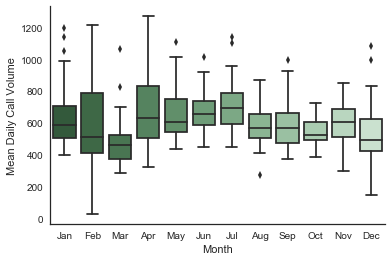
\includegraphics[scale=.4]{monthly_boxplot.png}
	\caption{Distribution of average daily call volume by month}
	\end{figure}

	\begin{figure}
	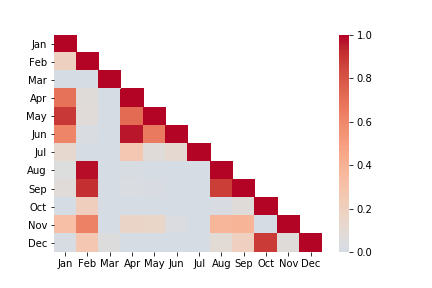
\includegraphics[scale=.4]{Heatmap.png}
	\caption{P-values resulting from t-test on daily call volume by month}
	\end{figure}

\paragraph{Call Volume by day of the week} can be compared in the boxplots in Figure 3.  Upon evaluation, call volume trends highest on Monday, then steadily decreases as the work week continues on.  The call center is not open on the weekend, so this could be a reason for the higher number of calls on Monday and Tuesday. Presumably, customers would call early in the week to address any issues that arose over the weekend.  A heatmap is shown in Figure 4, which emphasizes the statistically different mean for each pairing of weekdays.  The comparison of Wednesday and Thursday, according to this test, is the only pairing that does not exhibit statistically significant different call distribution from each other.

	\begin{figure}
	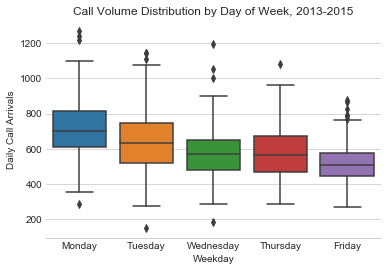
\includegraphics[scale=.4]{Daily_Call_Boxplot.png}
	\caption{Distribution of average daily call volume by weekday}
	\end{figure}

	\begin{figure}
	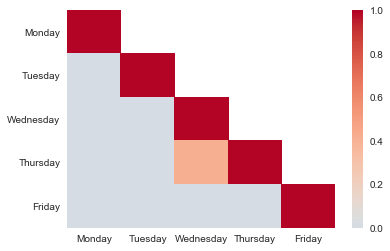
\includegraphics[scale=.4]{Daily_Heatmap.png}
	\caption{P-values resulting from t-test on daily call volume by day of the week}
	\end{figure}

\paragraph{Calls by department} were analyzed by two measures:  average duration and total volume.  Departments such as Solid Waste and Water Works had the highest call volumes, while Code Enforcement and the Mayor's Office had the longest average durations.  Given this incongruency, it is not immediately clear where the call center's resources should be focused.  As a more direct approach to the measure of total call volume, the total departmental call times were calculated.  This can be visualized in Figure 5.

	\begin{figure}
	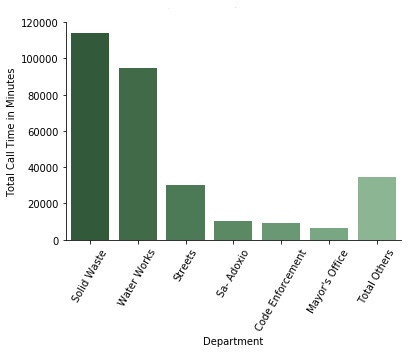
\includegraphics[scale=.4]{InkedCalls_Department_sim_LI.jpg}
	\caption{Total time spent on calls by top departments}
	\end{figure}

\paragraph{Calls by topic} were also analyzed by duration and volume.  When ranked by average duration, many obscure topics rose to the extremes.  Of the top 20 topics with the shortest duration, 19 consisted of less than three total calls.  Viewed as a percentage of the total 202,500 call dataset, these calls are such a small proportion that it would provide marginal insight to the city.  A similar, though less extreme, situation occurred when viewing topics with by duration.  This is be illustrated through a quantile-quantile plot for individual topics with percentile score for both average duration and total volume serving as the axes, which can be seen in Figure 6.

\par
In light of this exploration, it was determined that the most important results for the city to see included only topics composing a significant proportion of total calls.  When ranking by duration, only topics with total volume above the first quartile of total call volume were included, yielding results that could be viewed as more relevant to management.  Topics with long durations seemed to be centralized around complaints and billing issues, and topics with a short mean duration were mostly general information inquiries.  When analyzed in this manner, there is a 195 second difference between the mean durations of the longest and shortest topics.

\par
Topic volume was dominated by topics within many of the top departments identified earlier in Figure 1.  The top two highest volume topics, by a large margin, were “Miscellaneous Trash Information” and “Water Miscellaneous”.  This is reflective of positions of Solid Waste and Water Works in the departmental analysis.  In order to allow the city to effectively visualize this tandem effect, topics within the some of the busiest departments were plotted in an interactive scatterplot, as seen in Figure 7.  In this visualization, average call duration and total call volume serve as the axis, with glyphs used to differentiate between departments.  As the inset image illustrates, a zoomed view is necessary to more clearly see relationships between topics.  The Bokeh library allowed for this ability to be coded into the plot.


	\begin{figure}
	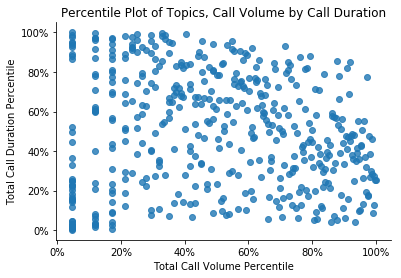
\includegraphics[scale=.4]{new_q-q_plot.png}
	\caption{\textbf{Quantile-Quantile Plot of Topics: Call Volume by Call Duration} \\
	Illustration of individual topics' disparity between call duration and quantity}
	\end{figure}

	\begin{figure}
	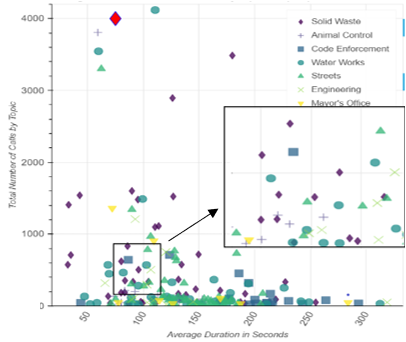
\includegraphics[scale=.6]{scatter_ready.png}
	\caption{\textbf{Scatterplot of Call Volume by Topic: The Busiest Departments} \\
		The diamond is not plotted to scale and represents two solid waste topics that exceeded the bounds of the plot}
	\end{figure}






\section{Visualization}


The above analysis yielded results showing trends for the call center by time, department, and topic.  This project was geared towards discovering trends, patterns, and insights; these were then provided to the city so that they could formulate specific questions based on the story that was told by this data.  In order to provide this to city management, a visualization dashboard was chosen as the most effective medium.  The Bokeh package was used to create interactive visualizations and allowed the final product to be packaged into a HTML file and sent to the call center management.  In all, the dashboard includes visualizations of:

	\begin{itemize}
		\item Pie chart of total call time by department
		\item Histogram of call volume by day of week, overlaid, with legend providing hide/show capabilities
		\item Bar charts of topics with longest and shortest average call durations
		\item Jitterplot of call volume by topic within top departments
		\item Bar chart of call volume by month
	\end{itemize}

These charts all utilize various implementations of Bokeh tools, such as HoverTool, BoxZoom, Pan, and checkbox interactivity.  By incorporating these interactions into the dashboard, the result is a more dynamic, engaging product that is simple to interact with for employees outside of the technical fields.  An image of the final dashboard can be seen in Figure 8, while a live link can be accessed at \textit{http://jdbul33.github.io/CallCenterDashboard.html}.

	\begin{figure}
	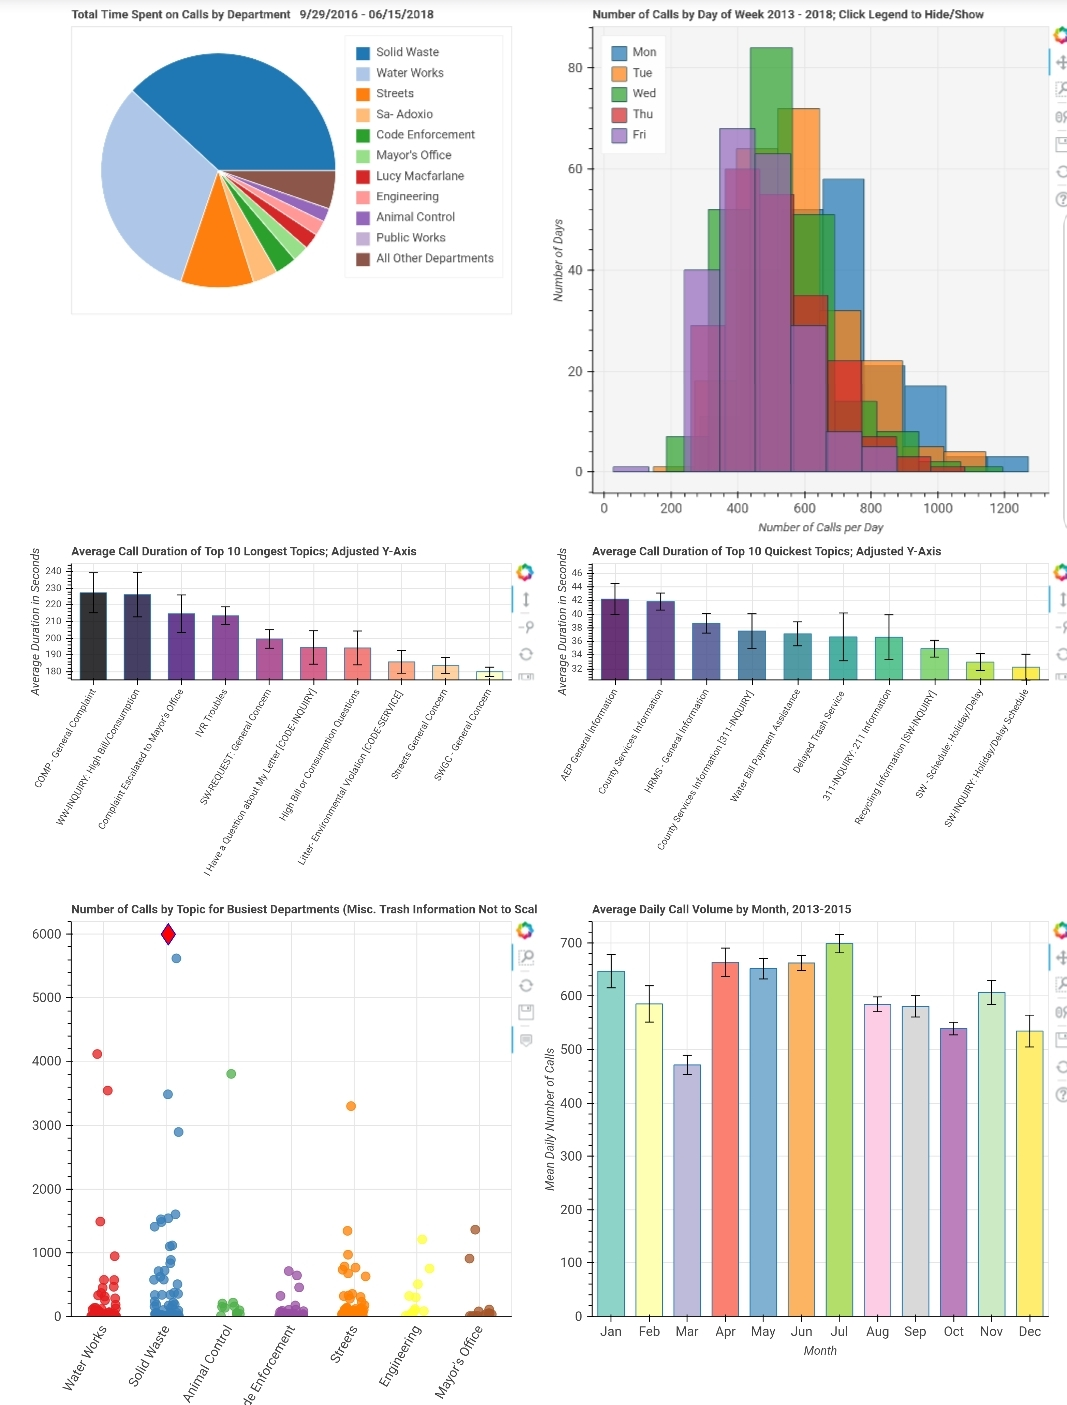
\includegraphics[scale=.4]{Dashboard.jpg}
	\caption{Static image of HTML-based dashboard delivered to the City of South Bend}
	\end{figure}



\section{Mathematical Model \& Simulation}

This data analysis laid the groundwork for a model and simulation that would be used to answer questions regarding staffing levels and hypothetical self-service line addition.  Additionally, the model was generalized so that it can be used for future questions and decision-making purposes.

	\subsection{Base Model}
The core model structure is based off the work of Mandelbaum in 2001\cite{mandelbaum}.  In his highly esteemed text, Mandelbaum lays out the basic schematic of a call center model.  His model illustrates the possible flow of a call, starting with its arrival until disposal, be that as a lost call or having completed successfully.  While simplistic by nature, the model covers all of the basic aspects of a call center in a sensible format that can easily by applied in Arena.  This model can be seen in Figure 9.  

	\begin{figure}[h]
	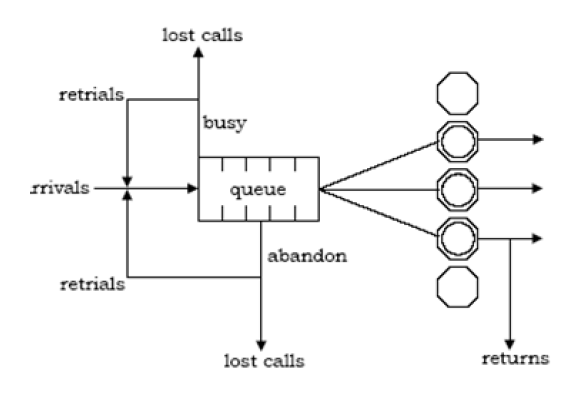
\includegraphics[scale=.45]{call_center_layout.png}
	\caption{Basic Operational Schematic of Call Center (Mandelbaum 2001)}
	\end{figure}

Mandelbaum's model identifies one avenue for arrivals (incoming calls) and three methods of disposal(lost calls due to busy signal, lost calls due to wait time, and completed calls).  It can be seen that the lost calls due to busy signals and the lost calls due to wait time both have retrial loops built in where some customers may immediately try to call into the system again and are treated as new arrivals for the sake of the simulation.  Completed calls also have the option to ``return", where they would immediately re-enter the system for whatever reason (perhaps an unresolved issue).  There is a single centralized queue before the calls are distributed among resources (operators).  At its core, this is a condensed high-level view of a call center model, designed so that it could easily be expanded as needed for specific analyses.

\subsection{Call Center Specific Model}
The model created for this analysis expands a great deal on the core model identified by Mandelbaum.  It adds three key features that are omitted in the original model: voicemails, operator breaks, and an alternate call flow for supervisor assistance.  Additionally, calls are assigned key attributes that determine their specific flow and timing throughout the simulation.  These key attributes include topic, language, and priority.  The hypothetical self-service option was added on to this expanded model for the relevant analysis.

	\paragraph{Voicemails}
	
In addition to arriving calls, voicemails are ``created" as soon as each simulation ``day" begins, so that the call center has all day to return those calls.  These are considered a lower priority item for the call center operators.  A constant number of voicemails were received by the call center immediately at the beginning of each simulated day to represent the voicemails that built up the night before.

	\paragraph{Operator Breaks}

To try and obtain more accurate results, the operator resources were given ``breaks" to better simulate potential slow downs due to operator time off. Break scheduling is different for full-time and part-time employees, so both were taken into account for the simulation.

	\paragraph{Supervisor}
	
Some calls were routed to a supervisor after speaking with an agent.  This supervisor resource then resolved the call, or passed it back to an agent.  This was added in an attempt to model actual call center behavior, where some callers may need assistance beyond a basic operator or may request supervisor assistance for a dispute. 

	\paragraph{Topic}

Calls are assigned a topic based on the distribution of topics in historical call center data.  In an effort to preserve the simplicity of the model while still utilizing past data, the top six departments (by total number of calls) were specified, with the remaining calls grouped into an ``other" category.  By assigning a topic, the simulation was be able to utilize the historical mean and standard deviation of those topics' call durations in order to more accurately replicate the call center.  The departments specifically included in the model account for 90\% of the total call volume in the original source data, while the ``other" category constitutes the remaining 10\%.

	\paragraph{Language}

Each call and voicemail is assigned a language of either Spanish or English.  The actual call center deals in both of those language, and it has Spanish-speaking operators available.  In order to reflect this, the model's resources all speak English, with some able to speak Spanish as well.  Therefore, arrivals are routed into two queues:  one for English, and one for Spanish.  Historical data regarding this distribution was not immediately available, so this is modeled as an estimated parameter that was generated from the population demographics of South Bend.

	\paragraph{Priority}

All incoming calls are assigned a medium priority by default and all voicemails are given a low priority by default (as they can be answered and returned as time permits).  After speaking to an agent, calls needing escalation to a supervisor are given the highest priority (in the event they need to cycle back through the queue again).

	\paragraph{Self-Service}

One of the purposes of this project was to evaluate the impact of adding a self-service option that would eliminate the need to speak to an agent for certain call topics.  This was added as an extension of the base model, but was run separately from the base model for the use of direct comparison of the results.  Depending on the assigned call topic, callers have the option to self-service, with multiple routes leading to the agent queue in the event the caller has trouble with self-service and needs an operator.


\section{Verification \& Validation}

	\subsection{Verification Techniques}

The model and simulation was verified using two primary techniques.  First, the model was tested and run in stages, using simplified or constant parameters.  For example, voicemails were not created and queues were eliminated in order to most simply ensure the call arrival and attribute assignment worked as expected.  A similar process was repeated with voicemails and excluding call arrivals.  Resources (operators and supervisor) were reduced to one at a time and stepped through in order to ensure proper call processing treatment.  

\par

The model was also verified by ensuring the output matched the estimated results produced from a static analysis.  As an example, this includes the comparison of the total number of calls, number of dropped calls, and number of operator breaks for a given simulation period.  With randomness removed from the simulation, it is possible to ensure the numbers produced from these processes are close to what is expected.
	
	
	\subsection{Validation Plan}
	
The model and simulation's results were ultimately validated using historical data.  Since several years' worth of call center data was available, the results of the base simulation were compared to this.  The number of call arrivals was created from the historical data, so this can be compared as well.  The operator schedule was provided by call center management, allowing for actual validation for these values.  Historical data also exists for percent of calls abandoned, which was also be directly compared.
	

\section{Simulation \& Results}

	\subsection{Verification \& Validation}
	
	  An average week of simulation yielded a total of 2,586 calls, with static analysis suggesting an average of 2,505.  The simulation also yielded the correct number of breaks given the number of full-time and part-time employees that worked on a given replication.  The static analysis was computed by taking the sum of arrivals from the arrival schedule (a Poisson distribution) with no regard for randomness.  These values affirm the results being generated from the simulation.  For validation purposes, historical data suggests a total of 2,650 calls per week.  Again, these numbers can be seen as affirmation for the purposes of this simulation.
	  
	  \par
	  
	  Similarly, the number of breaks taken for the simulation match both the static analysis (serving as verification) and the actual operator schedule (serving as validation).  Other key parameters, such as call duration and the number of voicemails created, matched what was expected.  Given this information, along with more intricate verification of the model during construction, provides confidence that the simulations performed were valid.
	  
	  
	\subsection{Number of Operators}
	
	An evaluation of the number of operators on schedule was the first question addressed through simulation.  For this experimentation, three primary metrics were evaluated:  number of calls abandoned (hang-ups), average operator utilization, and average waiting time.  The number of calls abandoned metric, it should be noted, is based on a completely estimated parameter which has calls that have spent over 15 minutes in the queue ``hang up."  This is set as a repeating manager in Arena that checks the queue every 5 minutes.  While this is not how hang ups are determined in real-life, it does provide call abandonment numbers that are in line with historical data.  Additionally, since it is consistent among these trials, it still serves as a useful measure of the impact of schedule changes.
	
	\par
	
	The base number of operators, taken from the provided schedule in Figure 4, serves as the control for this exploration.  From this starting point, additional full-time operators were added and subtracted to gauge the effect.  The effects of adding a specific part-time schedule or such was not evaluated, since it would require input from the city for a specific request.  However, these simulations are set up as such that a specific inquiry could be easily explored.
	
	\par
	
	The simulation was run with the base operator schedule, -1, +1, and +2.  Calls abandoned and operator utilization can be seen in Figure 10.  Both of these metrics reacted as expected, with less hang-ups and lower operator utilization as the number of operators increased.  Wait time was an interesting metric, in that it did not vary significantly at all with the change in operators, varying by 0.02 hours.  This can most likely be attributed to the customer patience parameter; as callers hang up, the queue advances.  It seems that over replications, this effect evens out regardless of the number of operators (within reason).
	
	\begin{figure}[h]
		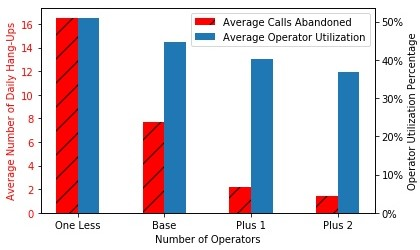
\includegraphics[scale=.5]{Inkednum_ops_plot_LI.jpg}
		\caption{Average daily number of abandoned calls and operator utilization percentage at different staffing levels}
	\end{figure}
	
	
	\subsection{Self-Service Call Option}

	The addition of a self-serve option was explored.  In this experimentation, only the percentage of eligible callers who choose the self-service option was adjusted; all other parameters were held constant.  Similarly, the number of operators was held to the current, actual schedule as provided by the call center.  This was done so in order to gauge the amount of consumers who adopt the self-serve option that would show a benefit to the call center.
	
	\par
	
	This experiment was run by utilizing Arena's Process Analyzer tool on the self-serve model.  The percent of customers (who have an eligible topic) was established as the control.  It was observed from 35\% to 85\%, in 5\% increments, as well as the literature-supported 67\% level.  Customer average wait time, number in the main operator queue, and operator utilization were set as the response variables.  Since this analysis is purely hypothetical, any sort of maximum self-service support threshold was not accounted for.
	
	\par
	
	Overall, this experimentation worked as expected.  As the number of callers who chose the self-service option increased, the wait time, queue length, and agent utilization all experienced linear decreases.  A visualization of the queue statistics can be seen in Figure 11.  Furthermore, the decrease in operator utilization can be seen in Figure 12.  It should be noted that in these trials, the graphs do show a definitive decrease in all metrics.
	
	\par
	
	The theorized 67\% utilization rate for the self-service option was then explored with an increase in mean call arrivals.  Through this analysis, it was observed that the self-service model with approximately a 20\% increase in total call arrivals exhibits agent utilization levels in range of the current state (base model) of the call center without the self-service option ($\approx$ 40\%).

\begin{figure}[h]
	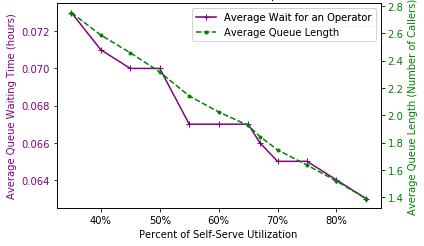
\includegraphics[scale=.5]{self_serve_results.png}
	\caption{Operator waiting queue statistics as a function of self-service adoption rates}
\end{figure}


\begin{figure}[h]
	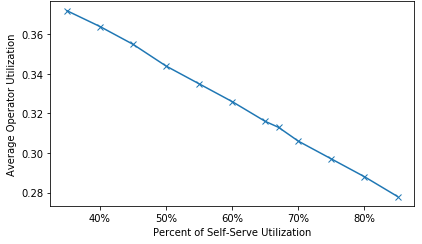
\includegraphics[scale=.5]{op_self_serve.png}
	\caption{Operator utilization in response to self-service adoption rates}
\end{figure}



\section{Discussion}

The results of both experiments provided clear metrics on which to base a decision.  First, it appears that the call center could add or remove a full-time operator without a substantial cost or customer service impact.  Removing an agent would change hang-ups per day from 8 to 16 (still a small percentage of the 400-500 daily calls received), and it would lead to a 6\% increase in agent utilization.  Given this, lessening the staffing levels by one full-time agent may well be a smart decision.  Adding one or two more operators reduces calls abandoned, but at a diminishing rate when compared to the loss of utilization.

\par

Secondly, the self-serve simulation experiment shows that operator utilization decreases in a linear fashion depending on the number of callers who can and do choose the self-service option, all else held equal.  Similarly, wait time and queue length decrease as well.  As expected, a self-serve option that even a small percentage of customers use could clearly make the case for removing one operator (as supported above, even without a self-serve option).  However, the true effectiveness of adding such a system would take into other factors, such as start-up and maintenance costs and customer education and marketing.  The extension of the self-service model analysis shows the increased amount of volume the call center can handle without necessitating hiring more staff.  Depending on the city's forecasts for the center, this may be a convincing argument to add this self-service system.

\par

Both of these experiments include estimated parameters, particularly the hypothetical self-service model.  As a result, neither of these experiments definitively answer/attempt to answer any of these questions until they are compared to internal data for accuracy.  Such data would replace estimates with more accurate numbers and distributions; then, a simulation could be run for a definitive question.









\section{Conclusion}

The goal of this paper was two-fold.  First, the analysis and presentation of data trends can be viewed as a successful high-level exploration.  Trends and points emerged from this analysis that will surely be of interest to call center management, while more insights can surely be found while interacting with the visualization dashboard.  For the city, this study should serve to identify areas of business interest within the context of these findings, which could then warrant further exploration with more specific questions.  For example, the city may want to see day-of-week trends for a specific topic, or they may seek to see how the number of calls queued relate to the number of calls abandoned.  These more specific questions would originate from a specific business need, which could perhaps be identified from this study.

\par

Secondly, this analysis resulted in the building of an accurate, historically validated model that was modified and used to provide results for two main questions.  While call centers are a frequently modeled system, this project was unique since it is based on an actual, operating center.  The inclusion of as much historical data as possible leads this analysis from the realm of theoretical into a practical and useful application.  A primary goal of this project was to create a model as similar as possible to the actual call center; this was achieved.  The questions explored, while simplistic in nature, would surely be of interest to city officials when it comes to budgets and annual planning.










\newpage
\clearpage
\pagenumbering{gobble}
\begin{thebibliography}{12}
	


\bibitem{baraka}
Hesham A. Baraka, Hoda Baraka, and Islam Hamdy EL-Gamily. 2013. Assessing call centers’ success: A validation of the DeLone and Mclean model for information system. \textit{Egyptian Informatics Journal} 14, 99-108.

	\bibitem{chen}
Chen, R-R., Chiang, Y., Chong, P.P., Lin, Y-H. \& Chang, H-K. (2011). Rough set analysis on call center metrics. Applied Soft Computing, 11, 3804-3811.

\bibitem{brown}
Lawrence Brown, Noah Gans, Avishai Mandelbaum, Anat Sakov, Haipeng Shen, Sergey Zeltyn, and Linda Zhao. Statistical Analysis of a Telephone Call Center: A Queueing-Science Perspective. \textit{Journal of the American Statistical Association} 100 (469), 36-50.

\bibitem{zhang}
Xiaowei Zhang, L. Jeff Hong, and Jiheng Zhang. 2014. Scaling and Modeling of Call Center Arrivals. In \textit{Proceedings of the 2014 Winter Simulation Conference (WSC ’14)}. IEEE Press, Piscataway, NJ, 467-485. 

	\bibitem{bapat}
Vivek Bapat and Eddie B. Pruitte Jr. 1998. Using Simulation in Call Centers. In \textit{Proceedings of the 30th.  1998 Winter Simulation Conference (WSC ’98)}. IEEE Computer Society Press, Los Alamitos, CA, 1395-1400.

\bibitem{saltzman}
Robert Saltzman and Vijay Mehrotra. 2007. Managing Trade-offs in Call Center Agent Scheduling: Methodology and Case Study. In \textit{Proceedings of the 2007 Summer Computer Simulation Conference (SCSC ’07)}. Society for Computer Simulation International, San Diego, CA, 643-651.


\bibitem{saltzman2}
Robert Saltzman and Vijay Mehrotra. 2001. A Call Center Uses Simulation to Drive Strategic Change. \textit{Interfaces} 31 (3). DOI: https://doi.org/10.1287/inte.31.3.87.9632.

\bibitem{mandelbaum}
Avishai Mandelbaum, Anat Sakov, and Sergey Zeltyn. 2001. Empirical Analysis of a Call Center. Technion Israel Institute of Technology, Israel.

\end{thebibliography}

\end{document}